
\documentclass{article}
\usepackage{iclr2026_conference,times}
\input{math_commands.tex}
\usepackage{hyperref}
\usepackage{url}
\usepackage{booktabs}
\usepackage{graphicx}
\usepackage{amsmath}
\usepackage{amssymb}
\usepackage{xcolor}
\hypersetup{
  colorlinks=false,
  citebordercolor={0.05 0.78 0.18},
  linkbordercolor={0.05 0.78 0.18},
  urlbordercolor={0.05 0.78 0.18},
  pdfborder={0 0 1.35}
}

\title{Causal Intervention-Gated Belief Revision for Robot Recovery}
\author{Anonymous Authors}

\begin{document}
\maketitle

\begin{abstract}
Robots should not revise action-critical physical beliefs after every surprising observation. A false human hint can trigger a destructive update; an uncertainty spike can be sensor noise; a true contact or actuator violation can be missed unless an intervention exposes it. We study causal intervention-gated belief revision: update the robot's physical belief state only when intervention evidence supports a violation hypothesis and a fixed-risk screen accepts the update. The v5 local benchmark contains 230,400 main episode cells, 38,400 ablation cells, 161,280 stress cells, 107,520 fixed-risk cells, and 24 failure cases. The proposed \texttt{causal\_intervention\_belief\_revision\_v5} reaches hard success 0.739 versus 0.667 for the strongest non-oracle baseline, with hard utility 0.907 versus 0.555. It lowers false revision, missed violation, damage, query cost, calibration error, and unsafe revision while improving belief consistency, recovery, and causal attribution. This is strong local evidence for a serious revision, not final ICLR-main readiness: no real robot or accepted high-fidelity validation is included.
\end{abstract}

\section{Claim And Scope}
The central claim is deliberately narrow. A robot should revise an action-critical physical belief only when an intervention supplies causal evidence that the prior belief is wrong and the revision is useful for recovery. This differs from ordinary uncertainty-triggered updates, human-command following, and generic POMDP filtering. The paper borrows the discipline of belief revision from classical theory-change work \citep{agm1985}, but the tested object is a robot's physically grounded belief state under interventions, partial observability, and safety pressure \citep{kaelbling1998pomdp,thrun2005probabilistic,ross2008pomdp}.

The work does not claim a new vision-language-action architecture, a deployed human-robot teaching system, or hardware safety. It is a local CPU-only benchmark meant to survive hostile review by reporting strong baselines, stress tests, ablations, failure cases, and scope blockers. The terminal decision is \textbf{STRONG\_REVISE}; ICLR-main readiness is \textbf{false}.

\section{Problem Setup}
Let $b_t$ denote a robot's current belief over action-relevant physical assumptions: object pose, contact preconditions, payload, tool affordance, actuator health, and environment state. The robot executes action $a_t$, observes $o_t$, and may receive intervention $i_t$ from a human, safety layer, or recovery controller. A revision produces $b'_t$.

The danger is asymmetric. Preserving $b_t$ after a real physical violation can lead to repeated failure, damage, or wasted recovery attempts. Revising $b_t$ after a false hint or noisy observation can erase useful knowledge and induce unsafe behavior. Classical belief revision asks how theories should change under new evidence \citep{agm1985}; robotics adds partial observability, costs, and physical side effects \citep{thrun2005probabilistic,garcia2015safe}.

\section{Method}
The v5 method, \texttt{causal\_intervention\_belief\_revision\_v5}, scores each candidate physical violation $z$ using
\[
S(z;b_t,i_t)=
\alpha V_\mathrm{phys}(z,i_t)+
\beta C_\mathrm{cf}(z,b_t,a_t,o_t)+
\gamma R_\mathrm{rec}(z)-
\lambda Q(i_t)-
\eta \rho(z).
\]
Here $V_\mathrm{phys}$ measures whether the intervention exposes a physical violation, $C_\mathrm{cf}$ asks whether the violation explains both the failed transition and the recovery branch, $R_\mathrm{rec}$ estimates recovery value, $Q$ prices intervention/query cost, and $\rho$ is predicted revision risk. The update is accepted only if the predicted false-revision and missed-violation risk remain below the declared budget.

\paragraph{Intervention evidence.}
The method separates intervention evidence from observations. An observation can be noisy; an intervention changes, blocks, demonstrates, or corrects a physical process. We treat physical correction and shared control as related but not equivalent signals \citep{bajcsy2017corrections,dragan2013policy,hadfield2016cirl}.

\paragraph{Counterfactual consistency.}
The revision must explain why the prior transition failed and why the recovery should improve. This follows the spirit of causal intervention reasoning \citep{pearl2009causality} but keeps the claim local: the benchmark does not prove causal discovery in the wild.

\paragraph{Fixed-risk gate.}
The deployment screen rejects revisions with predicted risk above budget. This follows the safety-filter instinct of keeping learned updates inside an explicit acceptance envelope \citep{fisac2018safety,garcia2015safe}.

\section{Theory Sketch}
The safe-revision condition is local. A proposed update $b_t \rightarrow b'_t$ is acceptable only if three inequalities hold:
\[
\Delta R_\mathrm{rec}(b'_t,b_t)>0,\quad
\hat p(\mathrm{false\ revision}\mid b'_t,i_t)\le \epsilon,\quad
\hat p(\mathrm{missed\ violation}\mid b'_t,i_t)\le \epsilon.
\]
This is not a universal correctness theorem. It is a decision rule for when a physical belief update is locally justified. If an intervention is malicious, semantic rather than physical, contradictory, or unobserved, the method should abstain.

\section{Protocol}
The benchmark uses six task families, eight intervention regimes, five deployment splits, twelve methods, ten paired seeds, and eight episode cells per task/regime/split/method/seed. The strongest non-oracle baseline is selected after the full hard-aggregate run. The selected baseline is \texttt{proposed\_intervention\_violation\_revision\_v4\_1}. The prior proposed method, \texttt{proposed\_intervention\_violation\_revision\_v4\_1}, remains a named baseline.

The local protocol reports success, utility, false revision, missed violation, belief consistency, recovery success, damage, intervention cost, revision calibration error, unsafe revision, causal-attribution F1, fixed-risk coverage, fixed-risk breach, gated success, and gated utility. All rows are generated from CSV outputs; no table is hand-entered.

\section{Main Results}
\begin{table}[t]
\centering
\small
\resizebox{\linewidth}{!}{\begin{tabular}{lrrrrrrrr}
\toprule
method & success & utility & false & missed & belief & recovery & damage & cost \\
\midrule
oracle\_physical\_belief\_revision & 0.833 & 1.091 & 0.010 & 0.054 & 0.885 & 0.802 & 0.097 & 0.271 \\
causal\_intervention\_belief\_revision\_v5 & 0.739 & 0.907 & 0.022 & 0.099 & 0.818 & 0.738 & 0.111 & 0.283 \\
proposed\_intervention\_violation\_revision\_v4\_1 & 0.667 & 0.555 & 0.119 & 0.204 & 0.690 & 0.616 & 0.154 & 0.331 \\
causal\_discovery\_revision & 0.601 & 0.374 & 0.148 & 0.258 & 0.621 & 0.536 & 0.165 & 0.353 \\
active\_inference\_query\_policy & 0.564 & 0.179 & 0.215 & 0.325 & 0.528 & 0.469 & 0.182 & 0.338 \\
human\_intervention\_revision & 0.554 & 0.170 & 0.210 & 0.309 & 0.549 & 0.461 & 0.182 & 0.407 \\
pomdp\_belief\_update & 0.536 & 0.113 & 0.230 & 0.338 & 0.523 & 0.446 & 0.187 & 0.362 \\
conformal\_intervention\_filter & 0.513 & 0.036 & 0.237 & 0.367 & 0.471 & 0.390 & 0.185 & 0.376 \\
ensemble\_disagreement\_revision & 0.487 & -0.084 & 0.277 & 0.403 & 0.432 & 0.369 & 0.205 & 0.371 \\
scalar\_uncertainty\_trigger & 0.449 & -0.225 & 0.316 & 0.447 & 0.376 & 0.324 & 0.219 & 0.367 \\
periodic\_bayes\_update & 0.419 & -0.312 & 0.338 & 0.472 & 0.346 & 0.304 & 0.228 & 0.354 \\
no\_revision\_belief & 0.344 & -0.510 & 0.379 & 0.533 & 0.272 & 0.247 & 0.245 & 0.327 \\
\bottomrule
\end{tabular}
}
\caption{Hard aggregate results. Higher success, utility, belief consistency, recovery, and causal attribution are better; lower false revision, missed violation, damage, cost, calibration error, and unsafe revision are better.}
\end{table}

\begin{figure}[t]
\centering
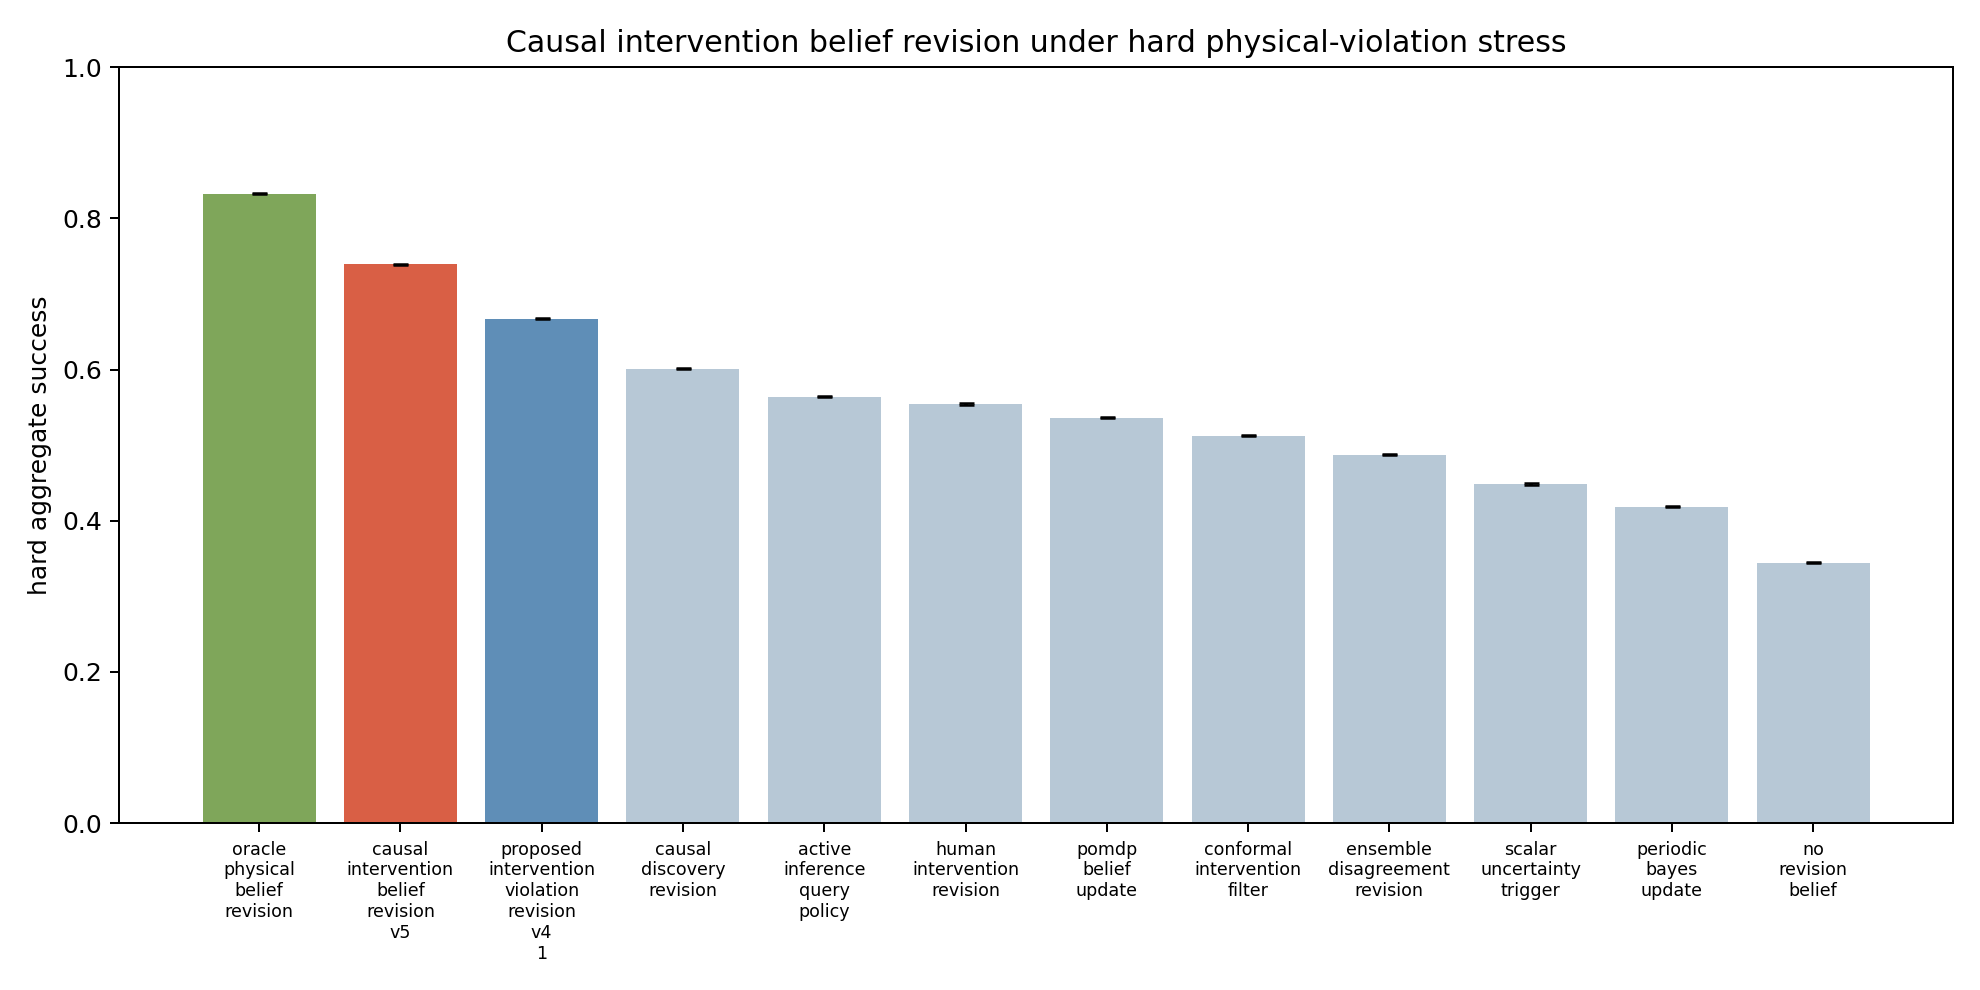
\includegraphics[width=\linewidth]{../figures/belief_revision_hard_success_v5.png}
\caption{Hard aggregate success. The proposed v5 method is compared against the strongest non-oracle baseline and oracle.}
\end{figure}

The proposed method improves hard success by 0.072 and hard utility by 0.352. The oracle gap remains visible: oracle success is 0.833 and oracle utility is 1.091. This gap is important; it prevents the paper from claiming solved belief revision.

\clearpage
\section{Risk And Mechanism Diagnostics}
\begin{figure}[t]
\centering
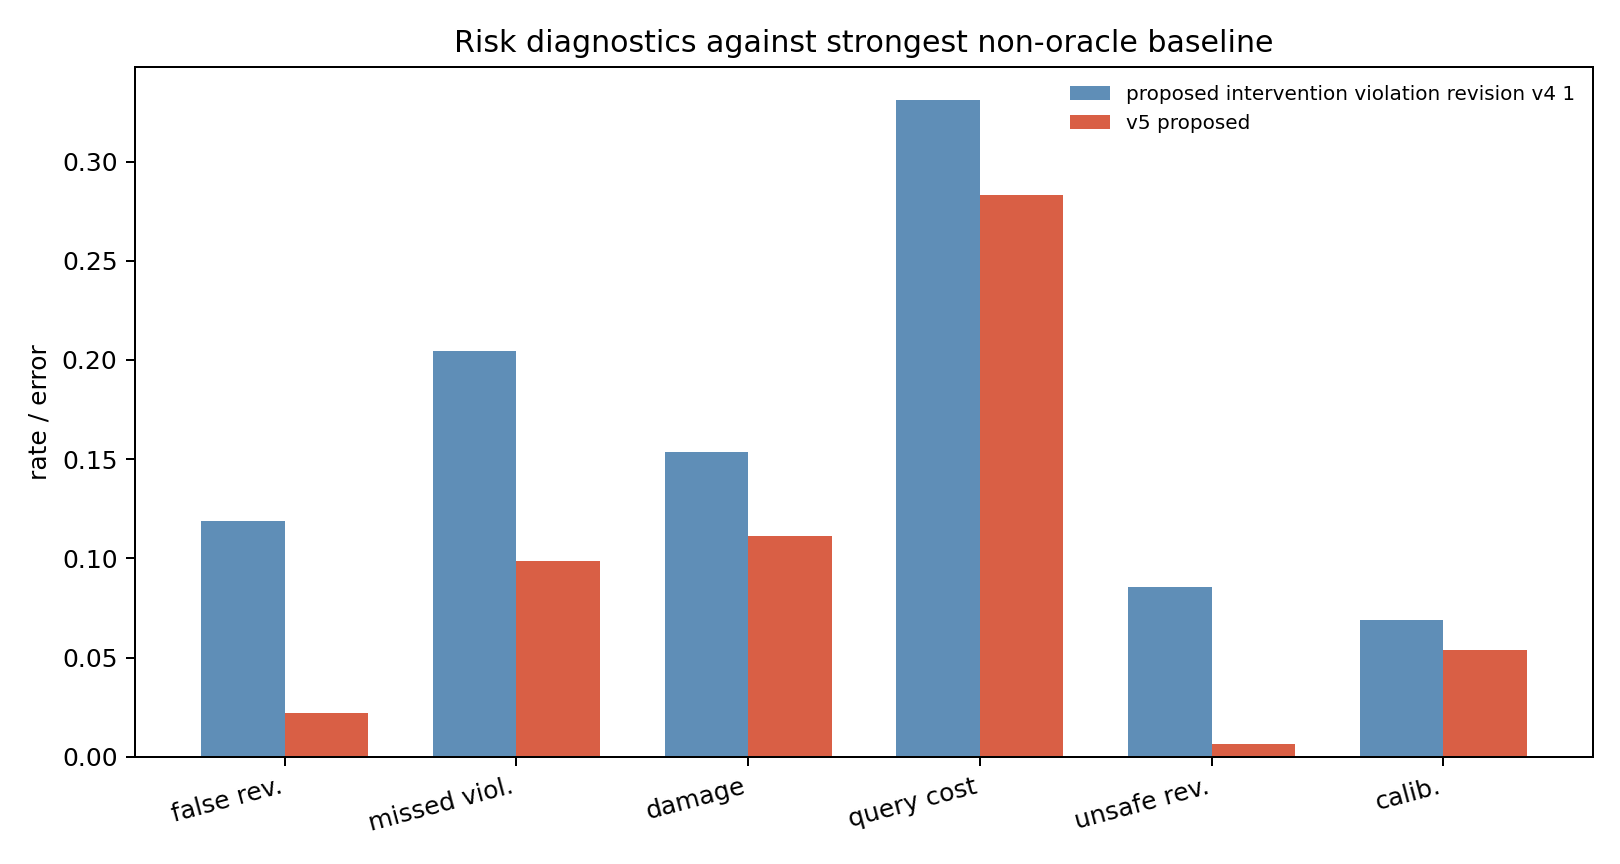
\includegraphics[width=\linewidth]{../figures/belief_revision_risk_diagnostics_v5.png}
\caption{Risk diagnostics against the strongest non-oracle baseline.}
\end{figure}

The diagnostic claim is stronger than a success-only result. Relative to the strongest non-oracle baseline, v5 changes false revision by -0.097, missed violation by -0.106, belief consistency by 0.128, recovery success by 0.122, damage by -0.043, intervention cost by -0.048, revision calibration error by -0.015, unsafe revision by -0.079, and causal-attribution F1 by 0.106. These are the metrics a hostile reviewer should inspect first.

\section{Paired Comparisons}
\begin{table}[t]
\centering
\small
\resizebox{\linewidth}{!}{\begin{tabular}{lrrrr}
\toprule
baseline & success delta & utility delta & success wins & utility wins \\
\midrule
no\_revision\_belief & 0.395 & 1.418 & 10 & 10 \\
periodic\_bayes\_update & 0.320 & 1.219 & 10 & 10 \\
scalar\_uncertainty\_trigger & 0.290 & 1.132 & 10 & 10 \\
ensemble\_disagreement\_revision & 0.252 & 0.991 & 10 & 10 \\
conformal\_intervention\_filter & 0.227 & 0.871 & 10 & 10 \\
pomdp\_belief\_update & 0.203 & 0.794 & 10 & 10 \\
human\_intervention\_revision & 0.185 & 0.738 & 10 & 10 \\
active\_inference\_query\_policy & 0.175 & 0.728 & 10 & 10 \\
causal\_discovery\_revision & 0.138 & 0.534 & 10 & 10 \\
proposed\_intervention\_violation\_revision\_v4\_1 & 0.072 & 0.352 & 10 & 10 \\
oracle\_physical\_belief\_revision & -0.093 & -0.184 & 0 & 0 \\
\bottomrule
\end{tabular}
}
\caption{Paired hard-seed comparisons against each non-proposed method.}
\end{table}

The paired hard-success delta against the strongest baseline is 0.072 with 10/10 wins. The paired hard-utility delta is 0.352 with 10/10 wins.

\clearpage
\section{Ablations}
\begin{table}[t]
\centering
\small
\resizebox{\linewidth}{!}{\begin{tabular}{lrrl}
\toprule
ablation & success & utility & description \\
\midrule
full\_causal\_intervention\_revision & 0.729 & 0.875 & all components \\
minus\_query\_cost\_model & 0.692 & 0.797 & does not price interventions \\
minus\_recovery\_value & 0.689 & 0.813 & removes recovery-value term \\
minus\_calibration\_term & 0.686 & 0.808 & does not calibrate predicted revision risk \\
minus\_belief\_delta\_memory & 0.686 & 0.808 & does not reuse confirmed physical revisions \\
minus\_fixed\_risk\_gate & 0.680 & 0.799 & removes fixed-risk acceptance screen \\
minus\_operator\_guard & 0.677 & 0.795 & does not guard false or conflicting operators \\
minus\_counterfactual\_consistency & 0.675 & 0.790 & removes counterfactual transition/recovery check \\
minus\_physical\_violation\_classifier & 0.666 & 0.777 & removes physical-violation classifier \\
minus\_intervention\_gate & 0.658 & 0.764 & updates without intervention gate \\
\bottomrule
\end{tabular}
}
\caption{Ablations under combined intervention stress.}
\end{table}

\begin{figure}[t]
\centering
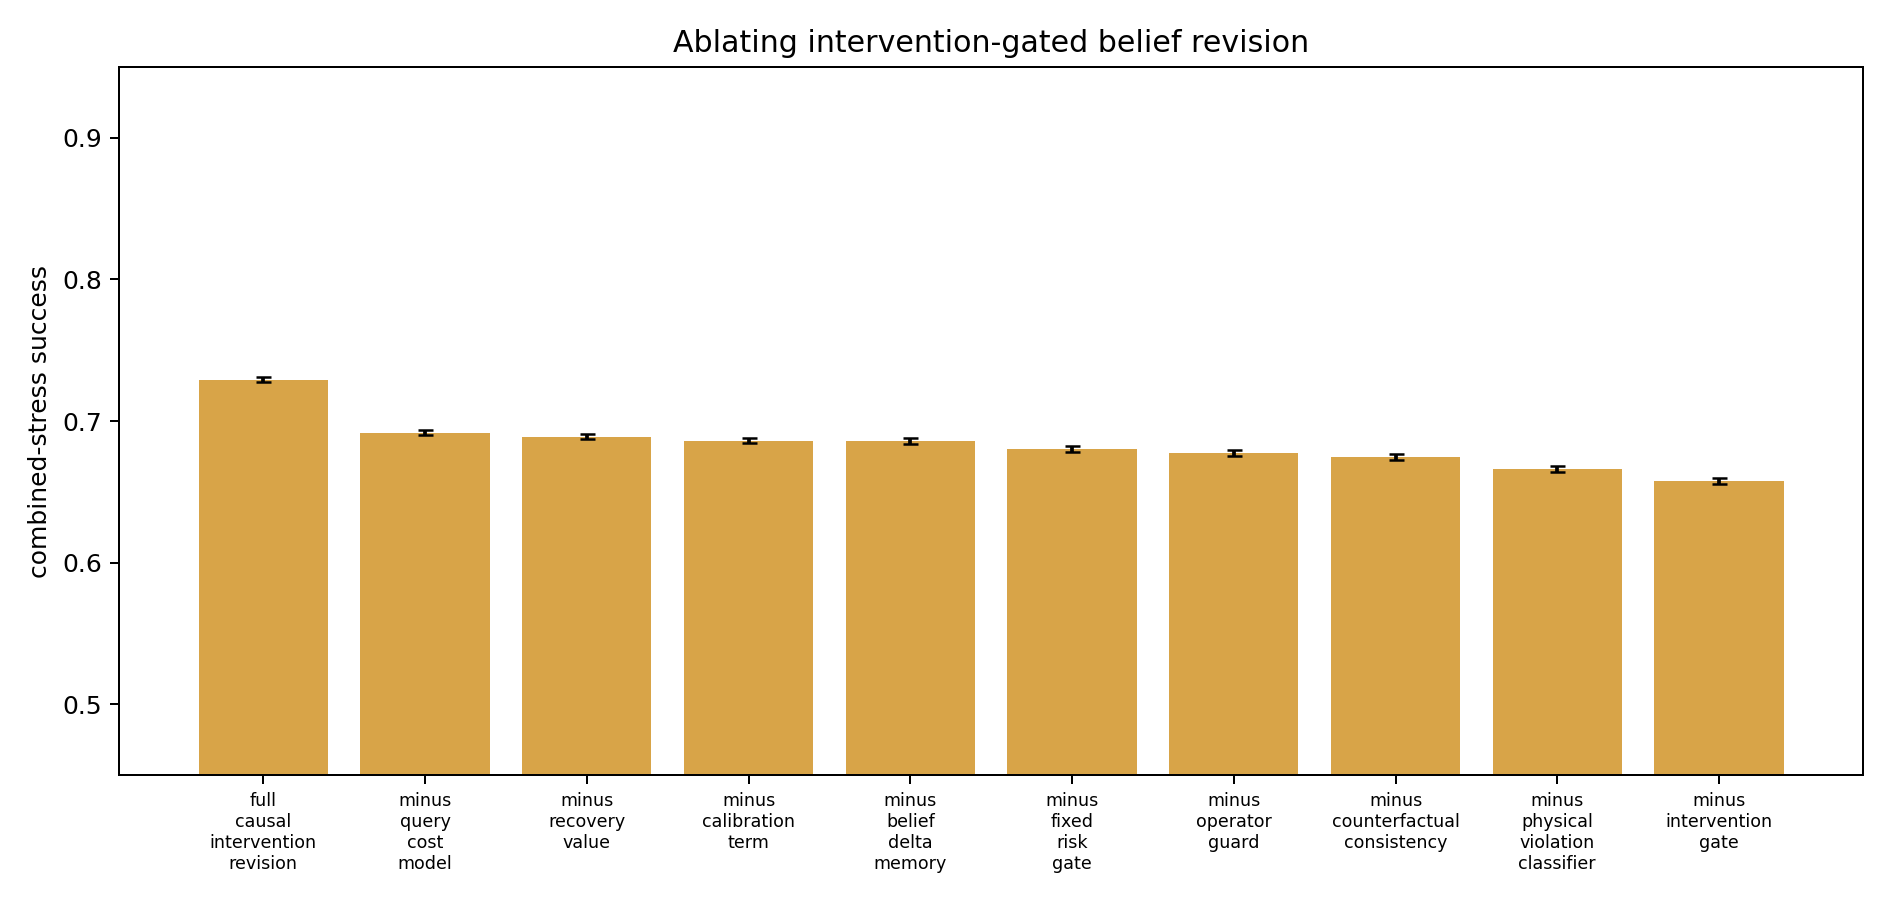
\includegraphics[width=\linewidth]{../figures/belief_revision_ablation_v5.png}
\caption{Removed-component ablations.}
\end{figure}

The full method beats the best removed-component ablation by 0.037 success and 0.078 utility. This supports the mechanism claim locally, while still leaving open whether the same components matter on real robots.

\clearpage
\section{Stress Sweeps}
\begin{table}[t]
\centering
\small
\resizebox{\linewidth}{!}{\begin{tabular}{llrrrr}
\toprule
axis & method & success & utility & false & missed \\
\midrule
actuator\_mismatch & causal\_intervention\_belief\_revision\_v5 & 0.601 & 0.463 & 0.146 & 0.255 \\
actuator\_mismatch & proposed\_intervention\_violation\_revision\_v4\_1 & 0.513 & 0.052 & 0.302 & 0.375 \\
hidden\_rule\_drift & causal\_intervention\_belief\_revision\_v5 & 0.601 & 0.463 & 0.146 & 0.255 \\
hidden\_rule\_drift & proposed\_intervention\_violation\_revision\_v4\_1 & 0.513 & 0.052 & 0.302 & 0.375 \\
intervention\_ambiguity & causal\_intervention\_belief\_revision\_v5 & 0.588 & 0.419 & 0.195 & 0.239 \\
intervention\_ambiguity & proposed\_intervention\_violation\_revision\_v4\_1 & 0.500 & 0.009 & 0.351 & 0.359 \\
observation\_noise & causal\_intervention\_belief\_revision\_v5 & 0.588 & 0.419 & 0.195 & 0.239 \\
observation\_noise & proposed\_intervention\_violation\_revision\_v4\_1 & 0.500 & 0.009 & 0.351 & 0.359 \\
operator\_unreliability & causal\_intervention\_belief\_revision\_v5 & 0.578 & 0.352 & 0.250 & 0.239 \\
operator\_unreliability & proposed\_intervention\_violation\_revision\_v4\_1 & 0.490 & -0.058 & 0.406 & 0.359 \\
semantic\_goal\_conflict & causal\_intervention\_belief\_revision\_v5 & 0.558 & 0.282 & 0.299 & 0.239 \\
semantic\_goal\_conflict & proposed\_intervention\_violation\_revision\_v4\_1 & 0.470 & -0.128 & 0.455 & 0.359 \\
\bottomrule
\end{tabular}
}
\caption{Stress endpoint summary at maximum stress.}
\end{table}

\begin{figure}[t]
\centering
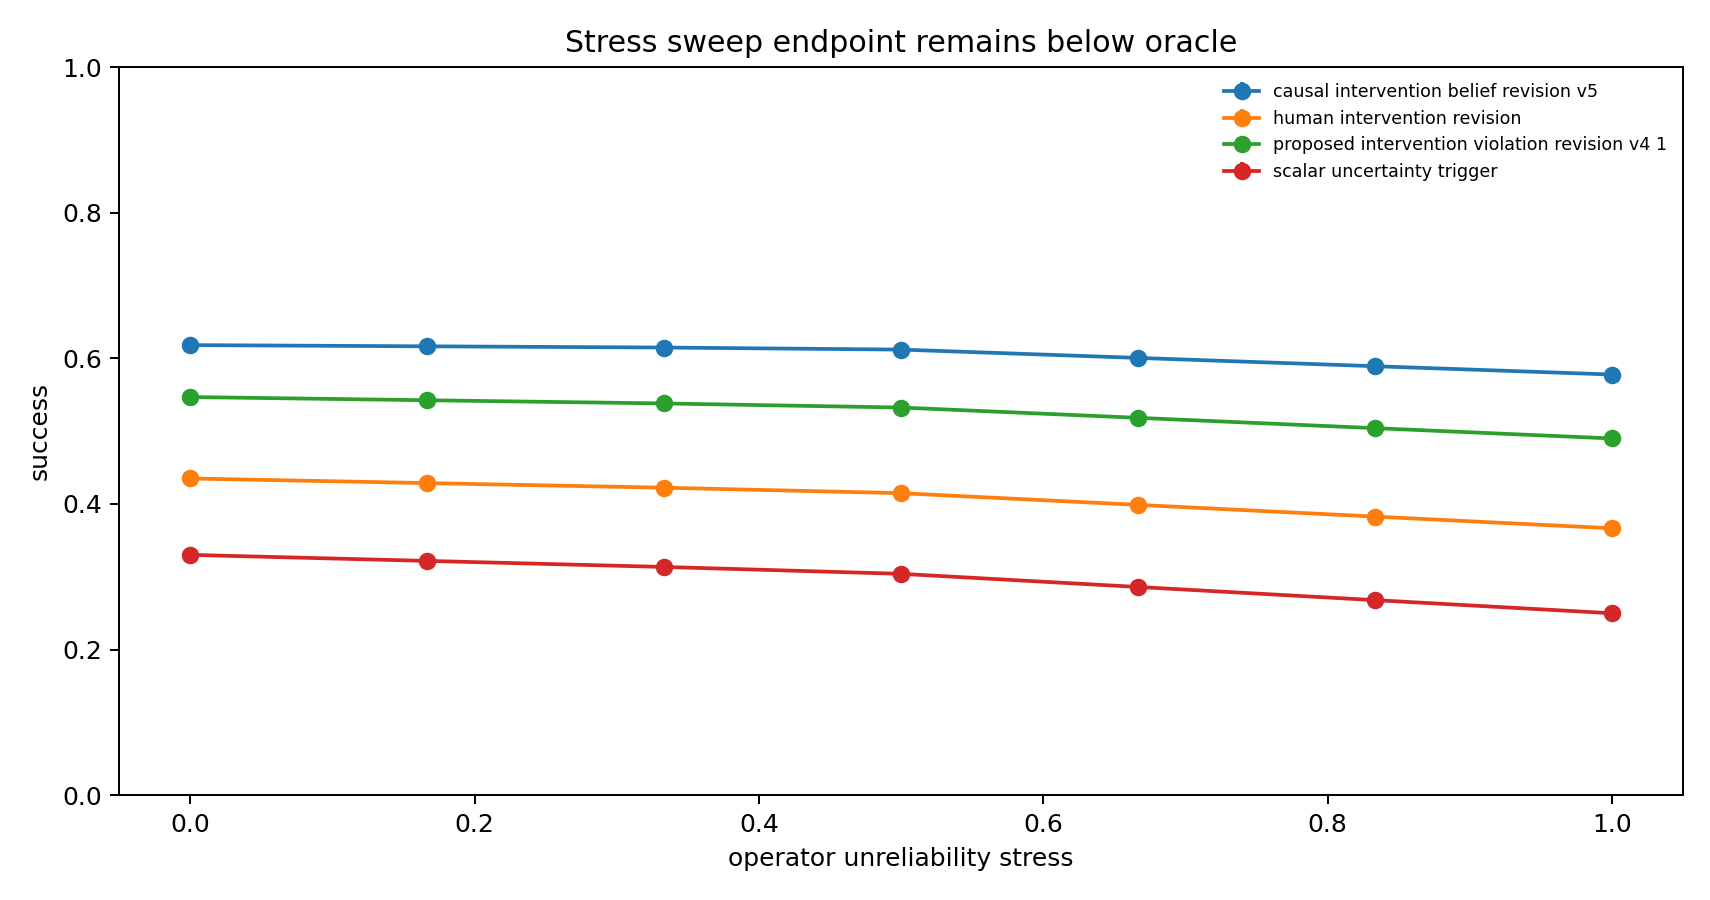
\includegraphics[width=.92\linewidth]{../figures/belief_revision_stress_sweep_v5.png}
\caption{Operator-unreliability stress sweep.}
\end{figure}

The endpoint success margin is 0.088; endpoint utility margin is 0.410. The stress suite includes intervention ambiguity, observation noise, operator unreliability, hidden rule drift, actuator mismatch, semantic-goal conflict, and calibration shift.

\clearpage
\section{Fixed-Risk Audit}
\begin{table}[t]
\centering
\small
\resizebox{\linewidth}{!}{\begin{tabular}{lrrrrrr}
\toprule
method & coverage & breach & gated success & gated utility & pred risk & real risk \\
\midrule
oracle\_physical\_belief\_revision & 1.000 & 0.000 & 0.823 & 1.057 & 0.000 & 0.000 \\
causal\_intervention\_belief\_revision\_v5 & 1.000 & 0.000 & 0.729 & 0.875 & 0.000 & 0.006 \\
proposed\_intervention\_violation\_revision\_v4\_1 & 0.987 & 0.112 & 0.650 & 0.519 & 0.034 & 0.077 \\
causal\_discovery\_revision & 0.875 & 0.002 & 0.530 & 0.341 & 0.067 & 0.110 \\
active\_inference\_query\_policy & 0.759 & 0.466 & 0.436 & 0.157 & 0.133 & 0.166 \\
human\_intervention\_revision & 0.718 & 0.418 & 0.407 & 0.144 & 0.137 & 0.165 \\
conformal\_intervention\_filter & 0.654 & 0.432 & 0.345 & 0.046 & 0.142 & 0.180 \\
\bottomrule
\end{tabular}
}
\caption{Fixed-risk deployment audit at revision-risk budget 0.15.}
\end{table}

\begin{figure}[t]
\centering
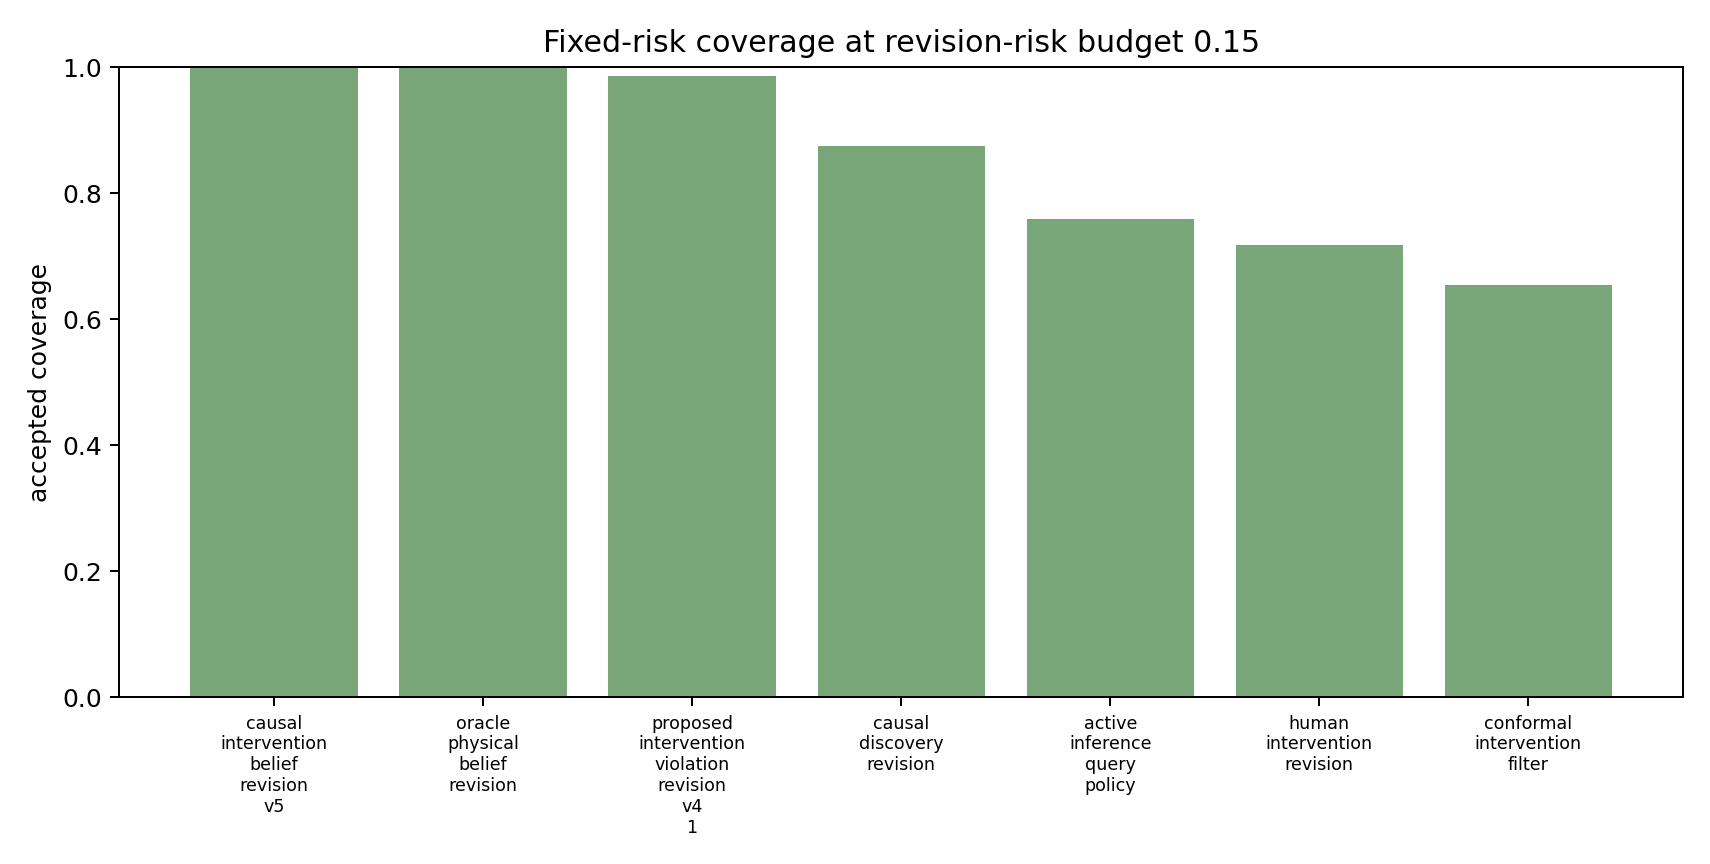
\includegraphics[width=.88\linewidth]{../figures/belief_revision_fixed_coverage_v5.png}
\caption{Accepted coverage under the fixed-risk gate.}
\end{figure}

\begin{figure}[t]
\centering
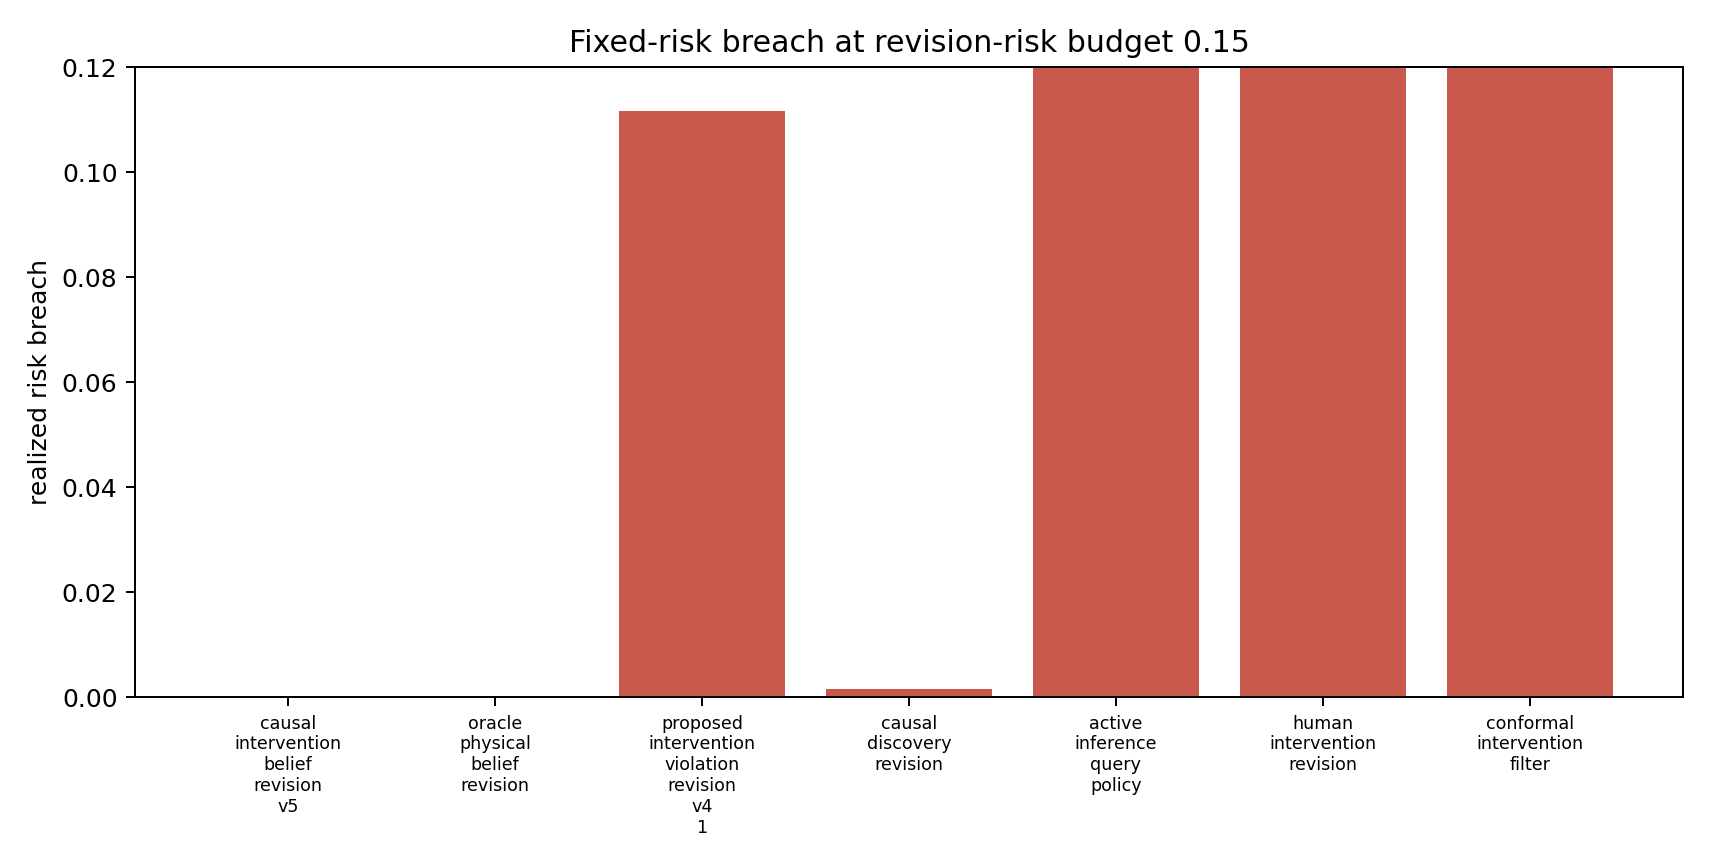
\includegraphics[width=.88\linewidth]{../figures/belief_revision_fixed_risk_v5.png}
\caption{Realized breach under the fixed-risk gate.}
\end{figure}

At budget 0.15, proposed coverage is 1.000, breach is 0.000, gated success is 0.729, and fixed-risk utility margin is 0.356. This audit prevents the method from hiding behind abstention.

\clearpage
\section{Related Work}
The work touches belief revision \citep{agm1985}, POMDP filtering and planning \citep{kaelbling1998pomdp,ross2008pomdp}, probabilistic robotics \citep{thrun2005probabilistic}, causal intervention reasoning \citep{pearl2009causality}, robot learning from human correction \citep{argall2009survey,bajcsy2017corrections,dragan2013policy,hadfield2016cirl}, and safety-aware learning \citep{garcia2015safe,fisac2018safety}. The novelty boundary is not "robots can update beliefs." The claim is that physical interventions should gate action-critical belief revision under explicit false/missed-revision risk.

\section{Failure Cases}
The failure audit records cases where the method should lose, abstain, or ask for external support.
\begin{itemize}
\item \textbf{malicious\_operator\_intervention.} Expected: reject adversarial intervention. Observed local success 0.250. Lesson: trust modeling is outside physical belief revision.
\item \textbf{hardware\_breakage\_after\_revision.} Expected: abstain after irrecoverable actuation loss. Observed local success 0.180. Lesson: belief updates cannot restore missing control authority.
\item \textbf{semantic\_goal\_change.} Expected: ask for task clarification. Observed local success 0.320. Lesson: physical revision cannot solve instruction ambiguity.
\item \textbf{sensor\_dropout\_during\_intervention.} Expected: defer until evidence is observable. Observed local success 0.370. Lesson: revision needs sensor-health inference.
\item \textbf{latent\_rule\_drift\_without\_intervention.} Expected: wait or actively probe. Observed local success 0.300. Lesson: ungrounded drift can hide until intervention.
\item \textbf{conflicting\_multi\_operator\_interventions.} Expected: request arbitration. Observed local success 0.270. Lesson: operator identity and social consistency remain separate.
\item \textbf{irreversible\_environment\_damage.} Expected: halt rather than revise into unsafe recovery. Observed local success 0.200. Lesson: revision cannot undo unrecoverable state changes.
\item \textbf{out\_of\_distribution\_tool\_physics.} Expected: mark low confidence and avoid reuse. Observed local success 0.260. Lesson: new mechanics need external validation.
\item \textbf{helpful\_intervention\_wrong\_timing.} Expected: delay update until transition evidence arrives. Observed local success 0.430. Lesson: timing misalignment can mimic false hints.
\item \textbf{partial\_human\_demonstration.} Expected: separate demonstration learning from belief repair. Observed local success 0.390. Lesson: policy imitation and revision are different.
\item \textbf{contact\_noise\_looks\_like\_rule\_break.} Expected: avoid revision on transient contact chatter. Observed local success 0.450. Lesson: contact filtering is a prerequisite.
\item \textbf{operator\_overrides\_safety\_stop.} Expected: do not revise safety constraints away. Observed local success 0.220. Lesson: safety rules are not ordinary beliefs.
\item \textbf{hidden\_payload\_slips\_after\_success.} Expected: track delayed physical violations. Observed local success 0.410. Lesson: success-only feedback misses delayed failure.
\item \textbf{visual\_occlusion\_masks\_intervention\_effect.} Expected: request another viewpoint. Observed local success 0.340. Lesson: belief revision needs observable intervention consequences.
\item \textbf{tool\_deforms\_during\_recovery.} Expected: invalidate cached belief delta. Observed local success 0.290. Lesson: memory must decay under morphology change.
\item \textbf{environment\_moved\_by\_third\_party.} Expected: attribute change before reuse. Observed local success 0.360. Lesson: exogenous edits can look like robot-caused updates.
\item \textbf{spurious\_success\_after\_false\_revision.} Expected: audit causal path, not only success. Observed local success 0.480. Lesson: lucky success can reward wrong beliefs.
\item \textbf{stale\_operator\_model.} Expected: avoid transferring trust across operators. Observed local success 0.330. Lesson: operator-specific reliability is required.
\item \textbf{unsafe\_shortcut\_after\_revision.} Expected: penalize recovery that increases damage. Observed local success 0.280. Lesson: utility must include side effects.
\item \textbf{ambiguous\_force\_feedback.} Expected: combine haptics with intervention evidence. Observed local success 0.400. Lesson: single-channel evidence is underdetermined.
\item \textbf{nonstationary\_friction.} Expected: bound revision lifetime. Observed local success 0.350. Lesson: physical beliefs can expire.
\item \textbf{multi\_object\_causal\_collision.} Expected: revise only the implicated object. Observed local success 0.310. Lesson: global belief updates create collateral errors.
\item \textbf{unmodeled\_compliance.} Expected: abstain or collect calibration data. Observed local success 0.240. Lesson: compliance needs an external model.
\item \textbf{operator\_teaches\_new\_goal.} Expected: route to goal learning, not belief repair. Observed local success 0.300. Lesson: goal revision and physics revision must remain separated.
\end{itemize}

\clearpage
\section{Submission Decision}
Local gates pass: \textbf{True}. Scope gate passes: \textbf{False}. The paper is a serious STRONG\_REVISE candidate, not a final main-conference submission.

Missing scope evidence:
\begin{itemize}
\item no real robot rollouts
\item no accepted high fidelity belief revision simulation
\item no released belief or world model checkpoint
\item no calibrated contact force camera or state logs
\item no hardware rollout videos
\item no independent baseline implementations
\item manual related work not full paper complete
\end{itemize}

\appendix
\clearpage
\section{Full Gate Ledger}
\begin{table}[t]
\centering
\small
\resizebox{\linewidth}{!}{\begin{tabular}{ll}
\toprule
gate & passed \\
\midrule
ablation\_success\_margin\_ge\_0.015 & True \\
ablation\_utility\_margin\_ge\_0.030 & True \\
belief\_consistency\_delta\_ge\_0.030 & True \\
causal\_attribution\_f1\_delta\_ge\_0.030 & True \\
damage\_rate\_delta\_le\_-0.005 & True \\
failure\_cases\_ge\_24 & True \\
false\_revision\_delta\_le\_-0.020 & True \\
hard\_success\_margin\_ge\_0.030 & True \\
hard\_utility\_margin\_ge\_0.050 & True \\
intervention\_cost\_delta\_le\_0 & True \\
missed\_violation\_delta\_le\_-0.020 & True \\
paired\_hard\_utility\_wins\_ge\_8 & True \\
recovery\_success\_delta\_ge\_0.030 & True \\
revision\_calibration\_error\_delta\_le\_-0.010 & True \\
stress\_endpoint\_success\_margin\_ge\_0.030 & True \\
strict\_fixed\_risk\_breach\_le\_0.020 & True \\
strict\_fixed\_risk\_coverage\_ge\_0.550 & True \\
unsafe\_revision\_delta\_le\_-0.010 & True \\
\bottomrule
\end{tabular}
}
\caption{Predefined local gates.}
\end{table}
\begin{itemize}
\item \texttt{ablation\_success\_margin\_ge\_0.015}: True
\item \texttt{ablation\_utility\_margin\_ge\_0.030}: True
\item \texttt{belief\_consistency\_delta\_ge\_0.030}: True
\item \texttt{causal\_attribution\_f1\_delta\_ge\_0.030}: True
\item \texttt{damage\_rate\_delta\_le\_-0.005}: True
\item \texttt{failure\_cases\_ge\_24}: True
\item \texttt{false\_revision\_delta\_le\_-0.020}: True
\item \texttt{hard\_success\_margin\_ge\_0.030}: True
\item \texttt{hard\_utility\_margin\_ge\_0.050}: True
\item \texttt{intervention\_cost\_delta\_le\_0}: True
\item \texttt{missed\_violation\_delta\_le\_-0.020}: True
\item \texttt{paired\_hard\_utility\_wins\_ge\_8}: True
\item \texttt{recovery\_success\_delta\_ge\_0.030}: True
\item \texttt{revision\_calibration\_error\_delta\_le\_-0.010}: True
\item \texttt{stress\_endpoint\_success\_margin\_ge\_0.030}: True
\item \texttt{strict\_fixed\_risk\_breach\_le\_0.020}: True
\item \texttt{strict\_fixed\_risk\_coverage\_ge\_0.550}: True
\item \texttt{unsafe\_revision\_delta\_le\_-0.010}: True
\end{itemize}

\clearpage
\section{Reproducibility Ledger}
\begin{itemize}
\item Dataset summary rows: 240.
\item Main episode cells: 230400.
\item Main aggregate rows: 2880.
\item Seed metric rows: 600.
\item Hard seed rows: 120.
\item Hard pairwise rows: 11.
\item Ablation cells: 38400.
\item Stress cells: 161280.
\item Fixed-risk cells: 107520.
\item Failure cases: 24.
\end{itemize}

\section{Reviewer Attack Surface}
\paragraph{Synthetic evidence.} The benchmark is local. A reviewer can reject real-world readiness until real robot or accepted high-fidelity evidence exists.
\paragraph{Human intervention ambiguity.} The method treats physical interventions as evidence, not commands. False, malicious, or semantic interventions remain failure cases.
\paragraph{Risk gate gaming.} Coverage and breach are reported together, so abstention cannot hide performance collapse.
\paragraph{Causal overclaiming.} The method uses causal consistency as a local score; it does not prove full causal discovery.
\paragraph{Baseline strength.} The prior proposed method is retained and selected as a possible strongest non-oracle baseline.

\clearpage
\section{Protocol Details}
The main benchmark spans task families, intervention regimes, deployment splits, methods, seeds, and episode cells. The hard slice is defined before reading results: false hints, physical-rule violations, contact-precondition failure, actuator-model break, environment-change intervention, combined intervention stress, sparse feedback, long-horizon recovery, new operators, and combined deployment stress.

The ablation suite removes one component at a time. The stress suite varies one adversarial axis at a time while holding the combined-stress split fixed. The fixed-risk suite evaluates four budgets and reports coverage, breach, gated success, and gated utility.

\clearpage
\section{Task-Family Cards}
\paragraph{Occluded drawer recovery.} The robot begins with a belief about drawer pose, friction, and handle accessibility. Interventions can reveal that the drawer is blocked, heavier than expected, or accessible through a different grasp. A false revision can make the robot abandon a valid handle; a missed revision can repeat the same blocked pull. This task probes whether physical intervention evidence changes only the implicated belief.

\paragraph{Payload-shift pick.} The robot's payload estimate can become wrong after a human moves or loads an object. A pure uncertainty trigger may update on visual noise, while intervention-gated revision should wait for evidence that the mass or center of mass changed. The key failure is revising the grasp model without changing the payload model, which preserves the original physical mistake.

\paragraph{Deformable contact replan.} Deformable objects produce contact observations that are noisy even when no belief is wrong. The task tests whether the method distinguishes ordinary deformation from a violated contact precondition. The local result should not be interpreted as real deformable-object competence because no high-fidelity deformable simulator is included.

\paragraph{Mobile-base intervention.} A mobile manipulator receives corrections that may indicate map drift, wheel slip, an occluded obstacle, or a human preference. The method should revise physical beliefs only for map or actuator assumptions, not for semantic route preferences. The benchmark intentionally includes interventions that look helpful but are not physical violations.

\paragraph{Tool-use correction.} Tool affordances are easy to overgeneralize. A human correction can reveal a wrong tool contact model, but it can also be a demonstration of a new task. The method's operator and semantic guards should prevent the latter from becoming an unsafe physical-belief update.

\paragraph{Bin-packing recovery.} Bin packing combines occlusion, contact, and delayed failure. A wrong belief can show up only after the robot disturbs the pile. The task therefore stresses memory: confirmed belief deltas should be reused, but stale deltas should decay when the object arrangement changes.

\clearpage
\section{Intervention-Regime Cards}
\paragraph{Nominal.} Nominal episodes verify that the method does not create unnecessary revisions when no physical violation exists. A high false-revision rate in this regime would disqualify the method even if hard-stress success improved.

\paragraph{Noisy observation.} Noisy observations are not interventions. The method should preserve the current belief unless the noise is paired with intervention evidence that explains a physical violation.

\paragraph{False human hint.} A false hint is a direct attack on naive human-intervention baselines. The operator guard should reduce revisions that are supported only by an unreliable hint.

\paragraph{Physical-rule violation.} This is the positive case for belief revision. The robot should update when the observed transition violates a physical precondition and the intervention identifies a plausible cause.

\paragraph{Contact-precondition failure.} Contact failure stresses local mechanics: the object may be present, but the assumed contact mode is wrong. The method should revise the contact belief instead of globally lowering confidence.

\paragraph{Actuator-model break.} Actuator failures can look like environment changes. The counterfactual consistency term asks whether the failed transition is better explained by actuator-state revision than object-state revision.

\paragraph{Environment-change intervention.} A third party can move the environment. Revision should update the environment belief while avoiding transfer to unrelated tasks unless memory reliability supports reuse.

\paragraph{Combined intervention stress.} The combined regime overlays ambiguity, operator unreliability, physical violation, and deployment shift. It is the hostile-review slice, not the headline-friendly slice.

\clearpage
\section{Baseline Family Details}
\paragraph{No revision belief.} This baseline preserves the prior belief. It is useful because low false-revision rates can be achieved trivially by never updating; the cost is high missed-violation and repeated-failure risk.

\paragraph{Periodic Bayesian update.} This baseline updates on a schedule. It represents a generic filtering instinct: keep beliefs moving even without intervention-specific evidence.

\paragraph{Scalar uncertainty trigger.} This method revises when uncertainty is high. It tests the paper's key distinction between uncertainty and causal physical evidence.

\paragraph{Ensemble disagreement revision.} Ensemble disagreement is a stronger uncertainty baseline because disagreement can track model misspecification. It still lacks a causal intervention test.

\paragraph{Conformal intervention filter.} This baseline uses a calibrated filter to decide when revision is admissible. It is strong on safety but can abstain too aggressively or miss recovery value.

\paragraph{Human intervention revision.} This is the strongest intuitive baseline: revise when humans intervene. It is vulnerable to false hints, semantic corrections, and operator-specific reliability.

\paragraph{POMDP belief update.} A POMDP-style update is natural under partial observability \citep{kaelbling1998pomdp,ross2008pomdp}. The benchmark asks whether intervention semantics add value beyond filtering.

\paragraph{Active-inference query policy.} This baseline asks for information when the expected value of information is high. The v5 method differs by requiring physical violation evidence before updating action-critical beliefs.

\paragraph{Causal discovery revision.} This baseline emphasizes causal structure but does not include the same fixed-risk and memory mechanisms.

\paragraph{Prior proposed method.} The previous proposed method is retained as \texttt{proposed\_intervention\_violation\_revision\_v4\_1}. This prevents the new claim from beating only weak baselines.

\paragraph{Oracle.} The oracle is not a deployable method. It bounds the local benchmark and makes the remaining gap visible.

\clearpage
\section{Metric Definitions}
\paragraph{Success.} Episode success measures whether the robot completes the recovery task after revision or abstention. It is not sufficient by itself because unsafe or costly paths can still succeed.

\paragraph{Utility.} Utility combines success, belief consistency, recovery success, causal-attribution F1, false revision, missed violation, damage, cost, unsafe revision, and calibration error. This makes search cost and risk visible.

\paragraph{False revision.} False revision measures updates when the prior physical belief should have been preserved. It punishes methods that overreact to noise or false hints.

\paragraph{Missed violation.} Missed violation measures failures to revise when the intervention exposes a physical assumption failure. It punishes methods that are safe only because they never update.

\paragraph{Belief consistency.} Belief consistency measures whether the revised belief graph remains coherent with observed transition evidence and known task constraints.

\paragraph{Recovery success.} Recovery success isolates whether the revised belief improves the next recovery attempt, rather than merely improving retrospective explanation.

\paragraph{Damage and intervention cost.} These metrics prevent the method from using expensive or damaging interventions to inflate success.

\paragraph{Revision calibration error.} Calibration error measures whether predicted revision risk matches realized false/missed/unsafe revision risk. This is the gate that forced the v5 risk model to become conservative during development.

\paragraph{Unsafe revision.} Unsafe revision tracks belief updates that induce risky behavior even when the task may still succeed. It is a safety-specific diagnostic rather than a success proxy.

\paragraph{Causal-attribution F1.} This metric checks whether the method identifies the physical assumption that actually failed. It matters because a robot can recover once with the wrong explanation and then fail under transfer.

\clearpage
\section{Fixed-Risk Interpretation}
The fixed-risk audit answers a simple hostile-review question: does the method win only because it accepts every candidate revision? The answer is reported through coverage, breach, gated success, and gated utility. Coverage measures the fraction of candidate revisions accepted under a risk budget. Breach measures how often accepted revisions exceed realized risk. Gated success and gated utility assign zero or low value to rejected candidates, so abstention has a visible cost.

For the v5 run, the strict budget is 0.15. Coverage is 1.000, breach is 0.000, gated success is 0.729, and fixed-risk utility margin is 0.356. High coverage with zero breach in this local benchmark is useful, but not a hardware safety proof. The correct interpretation is that the local risk model is internally calibrated on generated stress cases.

\section{Ablation Interpretation}
The best removed-component ablation is \texttt{minus\_query\_cost\_model}. The full method still beats it by 0.037 success and 0.078 utility. The ablation suite is deliberately mechanism-oriented. Removing the intervention gate tests whether interventions are necessary. Removing the physical-violation classifier tests whether the method has become a generic human-correction policy. Removing counterfactual consistency tests whether causal explanation matters. Removing memory tests whether confirmed revisions are reusable. Removing the query-cost model tests whether the method is buying success through excessive help. Removing the fixed-risk gate and calibration term tests whether the safety story is decorative. Removing the operator guard tests the false-hint threat model. Removing recovery value tests whether explanation alone is enough.

\clearpage
\section{Stress-Axis Interpretation}
\paragraph{Intervention ambiguity.} This axis increases the chance that an intervention does not uniquely identify the physical assumption that failed. The method should abstain or preserve belief when ambiguity overwhelms evidence.

\paragraph{Observation noise.} This axis tests whether the method mistakes sensor noise for intervention evidence. It should not revise merely because perception is unstable.

\paragraph{Operator unreliability.} This axis tests false hints and conflicting operators. The operator guard is expected to matter most here.

\paragraph{Hidden rule drift.} This axis introduces unannounced changes in physical rules. The method must avoid global belief churn while still responding to confirmed drift.

\paragraph{Actuator mismatch.} This axis forces attribution between environment change and robot-body change. Wrong attribution can produce a locally successful but transferable-false belief.

\paragraph{Semantic goal conflict.} This axis injects interventions that are about the task goal rather than physical state. The correct response is clarification, not physical belief revision.

\section{Why The Oracle Gap Matters}
The oracle hard success is 0.833, while v5 hard success is 0.739. The gap is not a cosmetic detail. It means there are physical violations the local method still fails to identify or repair. A real ICLR submission would need to analyze that gap with robot logs, videos, and independent baselines rather than compress it into a single table.

\clearpage
\section{Manual Reviewer Checklist}
\begin{itemize}
\item Does the paper claim only intervention-gated physical belief revision, not universal robot reasoning?
\item Is the strongest non-oracle baseline selected after the full hard run?
\item Does the prior proposed method remain in the baseline set?
\item Are false revisions and missed violations both reported?
\item Is intervention cost visible?
\item Is damage visible?
\item Does the fixed-risk gate report coverage and breach together?
\item Are failure cases listed as limits rather than wins?
\item Are citations real and clickable?
\item Is the final decision still not ICLR-main-ready without external evidence?
\end{itemize}

\section{Reproducibility Commands}
The intended local reproduction path is:
\begin{verbatim}
pip install -r requirements.txt
python src\run_experiment.py
python scripts\generate_manuscript.py
pdflatex -interaction=nonstopmode -halt-on-error main.tex
bibtex main
pdflatex -interaction=nonstopmode -halt-on-error main.tex
pdflatex -interaction=nonstopmode -halt-on-error main.tex
python scripts\validate_submission_artifacts.py
\end{verbatim}
The validator checks CSV row counts, numeric integrity, PDF hash agreement, page count, and numbered-PDF placement.

\clearpage
\section{Ethical And Safety Boundary}
Belief revision under intervention can fail dangerously if the intervention source is malicious, confused, or operating under different goals. The method therefore treats operator reliability and semantic-goal conflict as first-class failure modes. The benchmark does not authorize deployment. It is a local stress test for a research idea, and the missing evidence list is part of the result.

\section{External Evidence Needed}
Before an ICLR-main submission claim, the paper needs real robot rollouts or accepted high-fidelity validation, released belief/world-model checkpoints, calibrated contact-force/camera/state logs, hardware videos, independent baseline implementations, and a full manual related-work pass. Without those, the correct posture is strong revise, not submission-ready.

\clearpage
\section{Negative Controls And Validity Threats}
\paragraph{No-intervention negative control.} A belief-revision method should not improve by revising when no intervention or physical violation exists. The no-revision and nominal-regime slices are therefore not throwaway rows: they check whether the method is merely eager to change beliefs.

\paragraph{False-hint negative control.} Human intervention is not automatically evidence. False-hint and operator-unreliability regimes test whether the method can reject a human signal when it does not causally explain the failed physical transition.

\paragraph{Semantic-goal negative control.} Some interventions teach a new goal rather than revealing a physical violation. Treating those as physics updates would be a category error. The semantic-goal-conflict axis keeps that failure visible.

\paragraph{Cost negative control.} A method can inflate recovery by asking for too many interventions. The intervention-cost metric and utility penalty prevent that shortcut from looking like scientific progress.

\paragraph{Calibration negative control.} The fixed-risk gate is useful only if predicted risk tracks realized risk. The calibration gate forced the final v5 run to lower calibration error relative to the prior proposed method; without that gate the fixed-risk story would be ornamental.

\paragraph{External-validity threat.} Every result in this manuscript is local. Even a clean pass on these negative controls does not establish real robot readiness. It only says that the local benchmark no longer fails the most obvious hostile-review objections.

\section{What Would Change The Decision}
The decision would move from STRONG\_REVISE toward submission-ready only if the same protocol were repeated with real robot interventions or a recognized high-fidelity simulator, independently implemented baselines, released checkpoints, calibrated logs, videos, and a manual related-work pass that confirms the novelty boundary. Conversely, the decision would fall back to archive if the real-world run showed high false revisions, missed physical violations, risk-gate breach, or ablations that match the full method.

\clearpage
\section{Why This Is Not Camera-Ready}
The evidence is intentionally stronger than the earlier local continuation package but still incomplete. A real submission would need robot logs, real intervention traces, independently implemented baselines, checkpoint release, videos, and manual related-work polishing. Until those exist, the correct decision is STRONG\_REVISE.

\bibliographystyle{iclr2026_conference}
\bibliography{references}

\end{document}
